\section{Utilisation des ordinateurs Raspberry Pi et serveurs à l'école}

Dans cette troisième phase, nous remplaçons les 600 ordinateurs DELL T1700/3620 par des Raspberry Pi, reliés à 6 serveurs, et nous réitérons les manipulations dans \textit{openLCA} afin d’évaluer l’empreinte carbone de cette nouvelle configuration. L’objectif est de comparer les deux approches pour déterminer la solution la plus durable.

La consommation électrique totale de l’infrastructure composée des 600 Raspberry Pi et des 6 serveurs s’élève à :

\[
E_{\text{totale}} = 1{,}76 \times 10^4~\text{Wh}
\]

Cette consommation se répartit comme suit :
\begin{itemize}
    \item \textbf{48\,\%} provient des 600 Raspberry Pi, soit environ 8\,608~Wh.
    \item \textbf{26\,\%} est due aux 6 serveurs, soit environ 4\,705~Wh.
    \item Le reste de la consommation est attribué à l'électricité consommée indirectement en France pour le fonctionnement global du réseau et de l'infrastructure.
\end{itemize}

L’impact carbone total estimé pour un serveur est de 784,25~kgCO\textsubscript{2}~eq. La répartition de cet impact entre les différents composants est la suivante :
\begin{itemize}
    \item \textbf{2 GPU} : 7\,\%
    \item \textbf{3 disques durs (HDD)} : 6\,\%
    \item \textbf{2 cartes mères} : 30\,\%
    \item \textbf{8 barrettes de RAM} : 6\,\%
\end{itemize}

En ce qui concerne les Raspberry Pi, l’impact carbone moyen d’un seul appareil est estimé à 14~kgCO\textsubscript{2}~eq.



\subsection*{Comparaison avec les ordinateurs DELL T1700/3620}

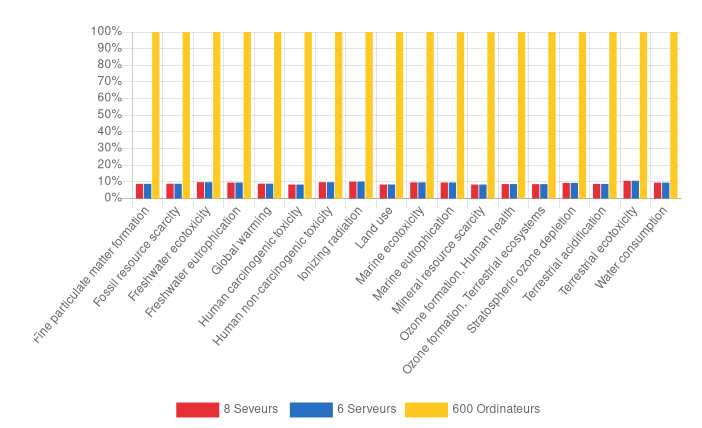
\includegraphics[width=0.8\textwidth]{images/imcomp.png}


Pour rappel, la configuration initiale avec les 600 DELL T1700/3620 présentait une consommation énergétique de \(8{,}17 \times 10^8~\text{Wh}\) et un bilan carbone global estimé à \(2{,}22 \times 10^5~\text{kgCO}_2~\text{eq}\) sur cinq ans.

En comparaison, la nouvelle solution composée de Raspberry Pi et de serveurs montre des résultats nettement plus favorables :
\begin{itemize}
    \item \textbf{Impact carbone des 600 Raspberry Pi} : \(600 \times 14 = 8{,}400~\text{kgCO}_2~\text{eq}\)
    \item \textbf{Impact carbone des 6 serveurs} : \(6 \times 784{,}25 = 4{,}705{,}5~\text{kgCO}_2~\text{eq}\)
\end{itemize}

\[
\text{Total (nouvelle solution)} = 8{,}400 + 4{,}705{,}5 = 13{,}105{,}5~\text{kgCO}_2~\text{eq}
\]

Cette solution alternative permettrait donc de réduire l’empreinte carbone d’un facteur supérieur à 16, en passant de plus de 222\,000~kgCO\textsubscript{2}~eq à environ 13\,100~kgCO\textsubscript{2}~eq. Cette réduction significative démontre l’intérêt environnemental d’une architecture informatique distribuée et légère, centrée sur des terminaux peu énergivores associés à des serveurs centralisés.

\subsection*{Limites de l’étude}

Cependant, cette étude présente certaines limitations qu’il convient de souligner. Tout d’abord, la composition exacte des ordinateurs utilisés (DELL T1700/3620, serveurs, Raspberry Pi) n’est peut-être pas parfaitement représentée dans notre modélisation, ce qui peut introduire des imprécisions dans les résultats.

Enfin, nous avons supposé que les pays producteurs des composants électroniques utilisaient une source d’électricité équivalente à celle de la France, notamment en matière de mix énergétique. Cette hypothèse, bien que pratique pour la modélisation, ne reflète pas nécessairement la réalité, certains pays pouvant recourir à des énergies plus carbonées, ce qui impacterait significativement le bilan final.

\subsection*{Avantages et inconvénients de chaque stratégie}

La stratégie consistant à équiper l’école de 600 ordinateurs DELL T1700/3620 présente un avantage certain en matière de confort pour les étudiants. En effet, chaque utilisateur dispose d’un poste de travail, disponible à tout moment, sans dépendance vis-à-vis d’une infrastructure réseau. Cette configuration garantit une puissance de calcul locale élevée et une réactivité optimale, ce qui est particulièrement appréciable pour les applications exigeantes.

Cependant, cette solution se révèle extrêmement énergivore et engendre une empreinte carbone très élevée, tant au niveau de la phase de fabrication que de la consommation électrique durant le cycle de vie des machines. Elle s’inscrit donc difficilement dans une démarche de développement durable.



La seconde stratégie, basée sur des terminaux légers (Raspberry Pi) couplés à des serveurs centraux, permet de réduire considérablement l’impact environnemental, aussi bien en termes d’énergie consommée que d’émissions de gaz à effet de serre. Elle est également plus flexible et plus économique à long terme.

Néanmoins, cette configuration repose fortement sur une infrastructure réseau performante et une gestion efficace des ressources serveur. En cas de forte affluence, si un grand nombre d’étudiants se connectent simultanément, des ralentissements peuvent survenir, affectant le confort d’utilisation et la fluidité du travail. De plus, la maintenance de cette architecture centralisée requiert une expertise technique spécifique.
\subsection*{Passage a 8 serveurs}

La conclusion finale reste inchangée, bien que l'augmentation de la consommation énergétique totale soit 
d'environ 12\,\%, car l'impact carbone global demeure environ 10\,\% inférieur à celui des ordinateurs DELL T1700/3620.
